\documentclass[../main]{subfiles}

\begin{document}

\chapter{Methodology}
In the next chapter there will be the explaination of the data pipeline that the project followed.
In particular, each subsection will focus on a specific task, except for the data visualization that has been used only when needed.

\section{Data Acquisition}
The used datasets are downloaded at runtime directly from the sources.
These datasets come directly from MovieLens' page, which provides 6 different datasets:
% TODO: think about, link README.txt

    \begin{table}[h]
        \begin{tabular}{|l | l|}
        \hline
        \textbf{Dataset} & \textbf{Features} \\
        \hline
        ratings.csv &  userId, movieId, rating, timestamp\\
        \hline
        tags.csv &  userId, movieId, tag, timestamp\\
        \hline
        movies.csv &  movieId, title, genres\\
        \hline
        links.csv &  movieId, imdbId, tmdbId\\
        \hline
        genome-scores.csv &  movieId, tagId, relevance\\
        \hline
        genome-tags.csv & tagId, tag\\
        \hline
        \end{tabular}
    \end{table}
        


where most of these datasets provides information for approximately 60000 films.
The links dataset provides two identifiers that allow to collect information from the IMDB and TMDB databases.
Thanks to the links' features, it has been possible to collect some more information on the running times of the films that could provide more insight into them.
Talking about the ground truth of the supervisioned models, the rating mean is missing. So the target feature will be computed during the pre-process phase thanks to the ratings dataset.
Further information about the features usage and the cardinality of the datasets will be discussed in the Pre-Process section.


\section{Data Pre-process}
In this section, will be discussed the Pre-Process phase for each of the above presented dataset.
In order to achieve a major clearity, the work on each dataset will be discussed in a specific subsection where the operation computed on them will be discussed.
\subsection{movies.csv}
Inside this dataset, the title and generes features contains multiple information. In particular, the title has been splitted in two part, where on one hand there's only the title name, and on the other, there's the year of the film production.
Since, the title name is a string, that doesn't add more information to a classic machine learning model, this feature has been converted into its length meanwhile, the production year just constitutes a new feature.
The genres feature contains a pipe separated list of a fixed possible values. Since the list is just saying if a film has a specific genre or not, to each film, all the fixed values has been added as a feature, and if a genre appears into the genres feature, that column will result into 1 that indicate the presence of that genre, 0 otherwise. At the end of this initial phase, the movies dataset looks like:
\begin{table}[h]
    \begin{tabular}{|l|l|l|l|l|l|l|l|l|}
    \hline
    \textbf{movieId} & \textbf{title\_len} & \textbf{year} & \textbf{action} & \textbf{adventure} & \textbf{animation} & \textbf{...}  & \textbf{Western} & \textbf{(no genres listed)} \\ \hline
    1                & 16                  & 1995          & 0               & 1                  & 1                  & ...           & 0                & 0                           \\ \hline
    \end{tabular}
\end{table}

In order to finish the data Pre-Process on this dataset, the data cleaning is required. First of all, there are some films where the year of the film production is missing.
Analyzing the distribuition of these \refname{fig:boat1} it is possible to see that the distribuition is right skewed, so the missing values can be filled with the \textbf{median}, as suggested during the lectures.
\begin{figure}[h]
    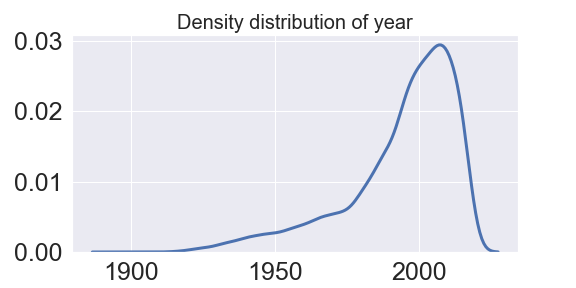
\includegraphics[width=\linewidth]{figures/original_year.png}
    \caption{Density distribuition of the year feature}
    \label{fig:boat1}
  \end{figure}
\section{Modeling}
\section{Performance Analysis}

\end{document}